\section{24" Log}
\subsection{10/2/2023}
In today's meeting, Collin, Chris, and Payton worked together to begin assembly of the 24" bot in reference
to the CAD file. They put together the 6 wheels and prepared every gear with its own shaft, collars, and teflon washers. Afterwards, they put together
the basic frame of the robot, consisting of the inner gearbox c-channel, along with cross-bracing to keep everything together.
Eventually, they attached 4 motors of the drivetrain and put together the outer c-channel for the gearbox, which would accomodate for a stacked rear motor in order to save space.
Now that the general frame of the robot was built, they are ending the meeting with putting together last minute tweaks regarding spacing of the wheels and moving their attention to assembling the drivetrain.
\subsection{10/3/2023}
Collin and Chris worked on adjusting the spacing of the gear-train so that the motors would have less of a load
with a lower amount of friction between gears. Then, they began to finish the cross-bracing between both sides of the robot to ensure
rigidity of the entire assembly. This allowed them to worry less on the drive binding up, while also making the frame of the bot much more stable.

\subsection{10/4/2023}
With the frame of the 24" bot assembled, Collin came in and placed the appropriate
gears and wheels, forming a drivetrain. He added bearings to the inner and outer c-channels of the gearbox and made sure that
every gear was meshing properly in order to prevent binding. Once he found the proper spacing and technique in order to keep
every gear and wheel perfectly aligned, he repeated this for the other side of the robot. Now that the
bot is driveable, they will begin putting their efforts into different subsystems of the assembly. Refer to \ref{fig:24_chassis}.
\begin{figure}
    \centering
    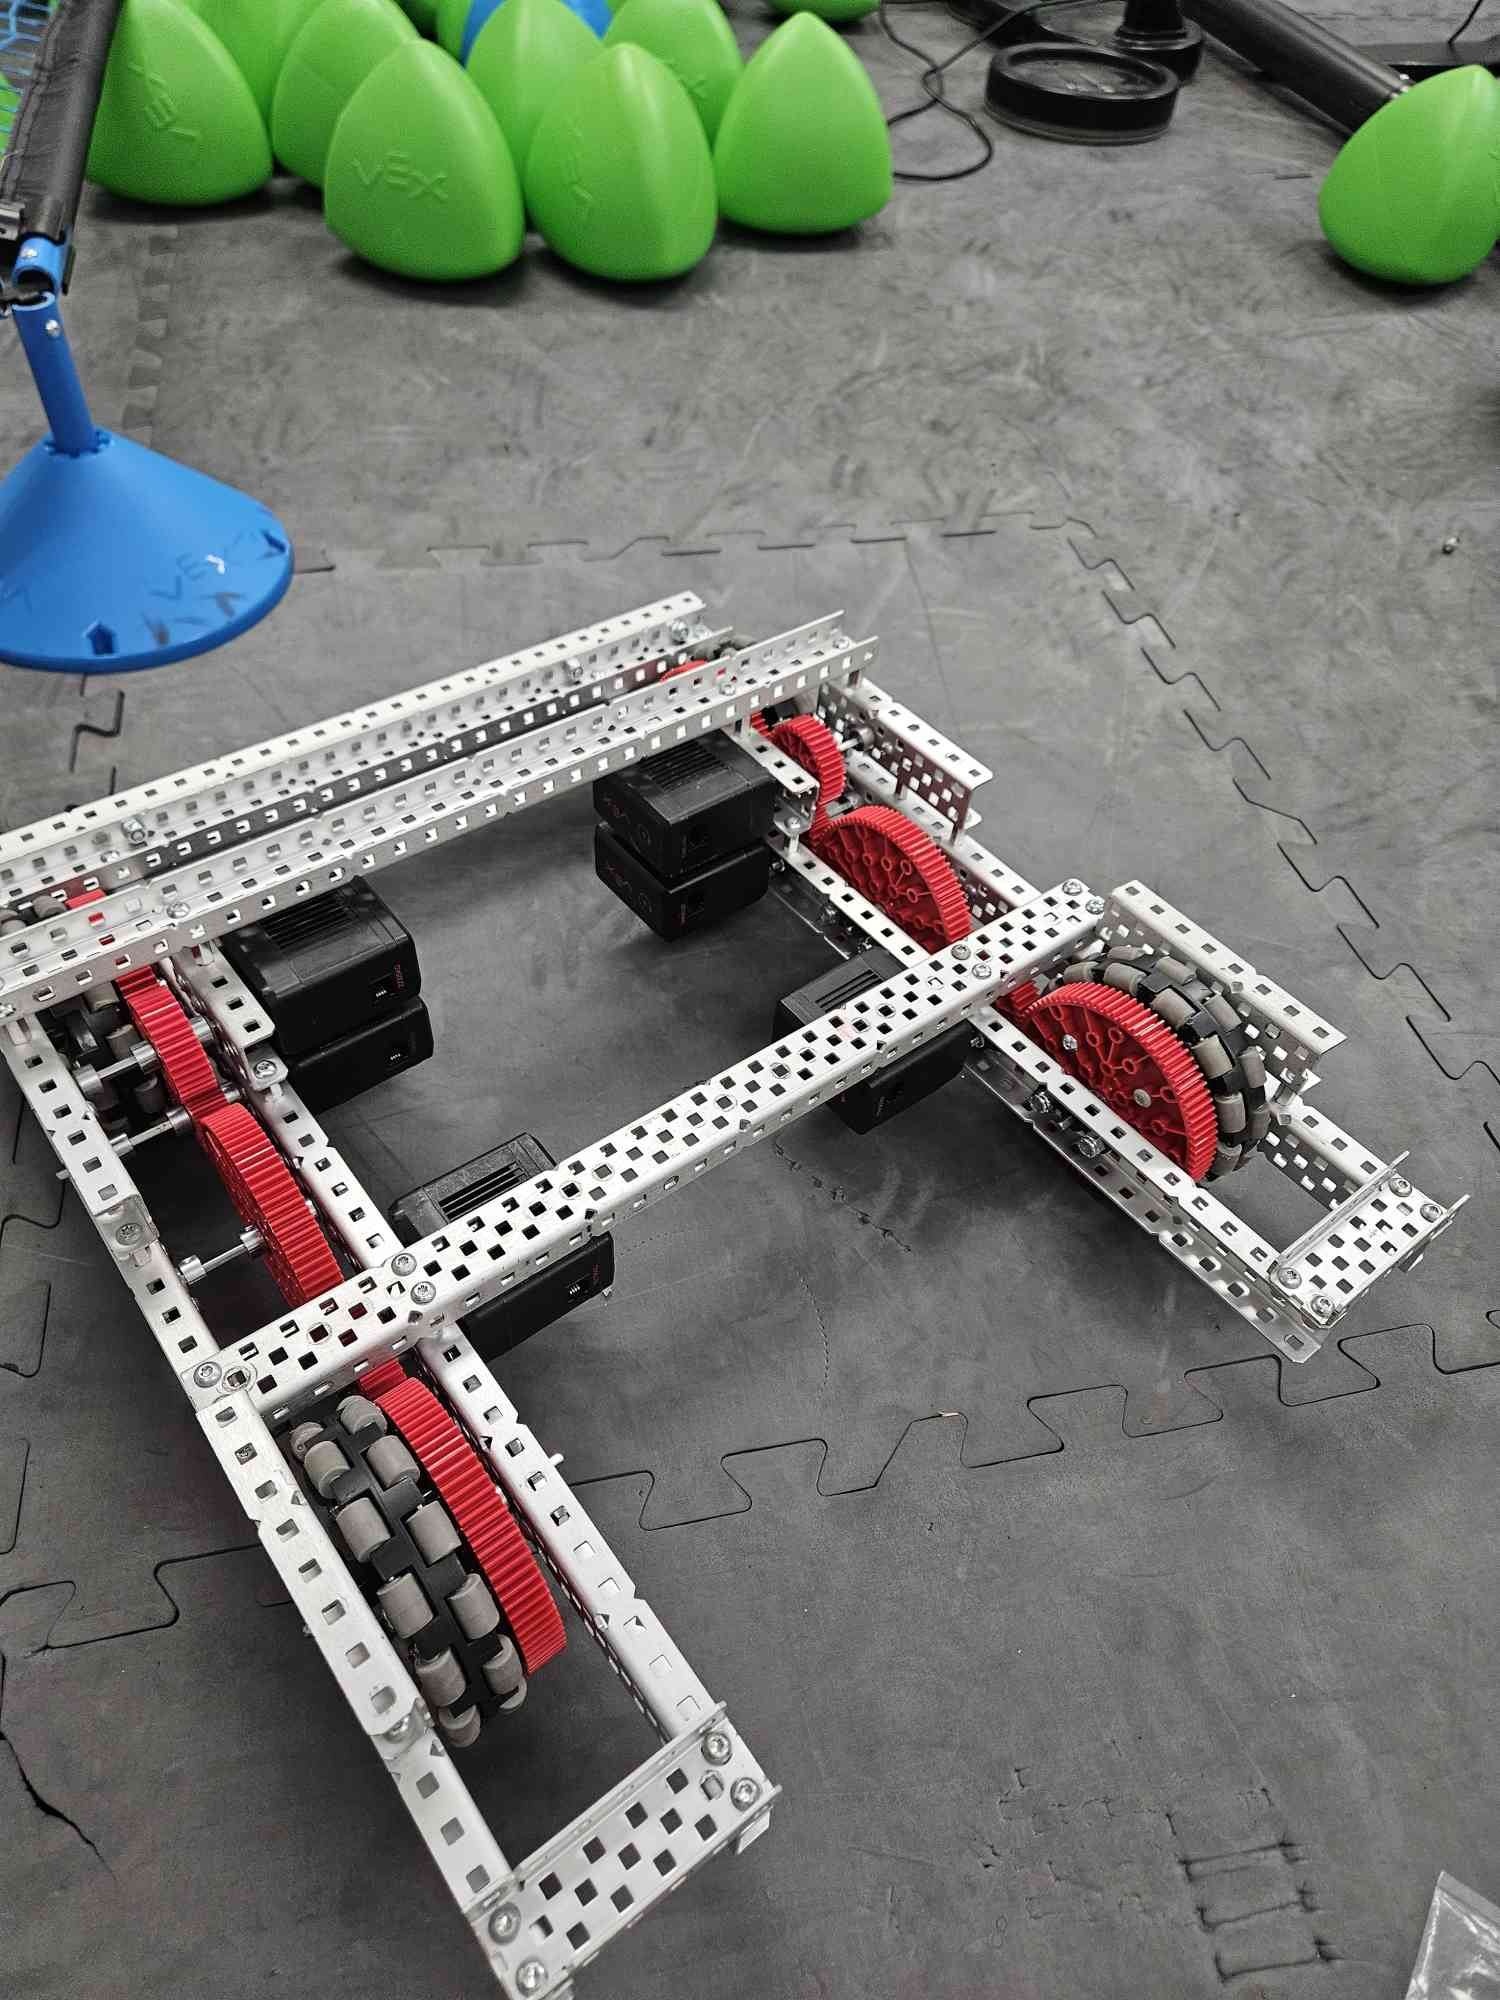
\includegraphics[width=0.5\linewidth]{images/october/24_chassis.jpg}
    \caption{The 24" chassis as of 10/4/2023.}
    \label{fig:24_chassis}
\end{figure}
\subsection{10/5/2023}
With what they had built now, it was time for testing the subsystems and perfecting small imperfections with their performance. Collin and Ryan worked on a drive motor and found it to be pulling too many watts, thus needing replacement. Then, Chris added a triangle brace comprised of standoffs to the outer piece of the intake. With the current edition of the CAD built, Collin began to design more cross-bracing and custom 3D printed pieces to keep the
intake control assembly aligned. He also updated the wing and skirt design in order to prevent possession calls of tri-balls.
\subsection{10/7/2023}
After everything with the drive train was wrapped up, there was nothing left on the CAD to build, so Collin began
to design a wing mechanism.
\subsection{10/9/2023}
As juan developed a way to retract and extend the intake assembly, Collin came in and replicated what he designed onto the 24".
This allowed the bot the ability to reach and intake tri-balls from the loading zone, while also retracting in order to stay within size constraints.
\insertimage{images/october/Intake_controller.jpg}{0.2}
\subsection{10/13/2023}
While the CAD was being worked on, Everett and Preston added another intake controller to the other side of the bot.
They did this so that the intake would retract evenly and not bind up as it would be used a great deal especially during autonomous. They also figured out that the speed the intake
moves at was far too slow. In order to safe space from forming a gear ratio, they decided to replace the green motor cartriges to blue, which run at a faster RPM.

\subsection{10/16/2023}
In the bot's current state, it is now time to begin testing designs for a flywheel. Ryan, Preston, and Everett worked on a design iteration that would test an elevated flywheel that makes contact with the top of tri-balls. Collin conceptualized a design that preserves space, in which the flywheel assembly is closer to the chassis, possibly allowing the 24
to pass under the low-bar of the field.
\insertimage{images/october/Flywheel_concept.jpg}{0.2}
\subsection{10/19/2023}
Today, Chris, Collin, and Payton began assembly of different subsystems of the robot. They found the correct sizing for the intake that would stay within 24" and critiqued the design from the CAD.
Collin also started testing different designs of the wing retraction mechanism. More bracing and support for these subsystems were added in order to keep building upwards for an intake control motor. Once the intake, wing mechanism, and intake control motor were completed, they began going over possible designs for a flywheel that would shoot the tri-balls across the field.

\subsection{10/28/2023}
Juan had already conceptualized a flywheel assembly by building on top of the intake control mechanism, so Collin adapted this design and made it cater to the larger bot's size. Later, Chris came and finished the job on the 
flywheel assembly after Collin had added c-channels in the correct position. Shortly after, the flywheel was built and they began to program the motors in the code to begin speed testing.
\insertimage{images/october/Flywheel_finished.jpg}{0.2}
\subsection{11/01/2023}
After a break to tend to studies, Collin and Chris came back and mirrored the intake control mechanism to the other side of the chassis. Without adequate bracing for the outer hub that holds the motor shaft, Collin went to design a piece to be 3D printed in inventor that would provide bracing and help align the tower in which the motor was mounted.
\subsection{11/02/2023}
The next day, Chris and Collin looked to tuning the intake of the robot and decided along with Juan and Hunter that a blue cartridge was better for the motor. This would help to intake tri-balls faster and more efficiently.
\subsection{11/09/2023}
After noticing a considerable lack of power with the intake, Collin and Chris concluded that is was most likely due to the high-strength shaft creating friction. They experimented with different ways to mount the banded sprockets
that would contact the tri-balls, including screw-joints and a low-strength shaft running through them. Ultimately, it was decided that returning to the high-strength shaft would be the best course of action, but they had to 
locate where the majority of friction was coming from.
\subsection{11/10/2023}
Chris and Collin eventually decided to change the mount for the high-strength shaft and bearings to reduce friction. The intake was now able to match-load quite well, although match-play would hold more problems that would need to be solved later on.
\insertimage{images/november/Intake_old.jpg}{0.1}
\subsection{11/16/2023}
After a short break, Braden had given us variable speed controls for the flywheel that we could test along with adding controller binds for the intake control mechanism. Collin began to work more with the pneumatic wings in which he 
decided there would need to be a lot more bracing in order to avoid deformation, knowing that a lot of force would be acting on this subsystem.
He then went on to CAD a 3D printable brace that would extend from the wing mounts to the chassis, ensuring that the force would be more evenly dispersed.
\subsection{1/19/2024}
Following Christmas break, the team got back together and bought more blue cartridges, so that we
 could put them in place for the green cartridges in the flywheel assembly, so that we could run the flywheel at higher RPM's, allowing us to shoot tri-balls farther.
\subsection{1/21/2024}
Today, in interest of saving space and cable management of the robot, Chris re-routed all motor cables to a new brain location, 
along with mounting the battery in a safer location. This way, we could minimize the space we were using as the bot is becoming more dense with further building.
\subsection{1/28/2024}
Ryan used the CNC machine to cut out the CAD renditions of the wings and skirt for the bot. Collin got these and mounted them to the wing bar and realized that the force it takes to prop
 the bot on the middle barrier was far too much for regular 1/8" ABS to handle. Aside from this, though, Collin did more work on mounting pneumatic actuators and running the tubing that would supply air to the double-acting pistons for the wings. This brought on a redesign for the skirt, along with the wing piece. Collin designed something more 
 similar to a sled that would lift the bot over the barrier as it runs into it. Afterwards, more tuning was done to the flywheel, such as adding rubber heads that are spaced to where they 
 make contact to the tri-balls before hitting the flywheel. This was done in order to create more compression on the balls as they shoot out from the bot. 
\insertimage{images/february/Sled.jpg}{0.2}
 \subsection{2/1/2024}
Following up on the match-loading capabilities of the intake, Chris began testing with cross-braces on the 
front end of the bot so that tri-balls would be held with more compression as they are brought up to the flywheel. In addition to this, a brace that was previously designed was 3D-printed that spanned between both sides of the intake.
Collin also began constructing a new mounting position and brackets for the wing assembly. This would conserve space and allow the pistons to have more leverage when deploying.  
\insertimage{images/february/New_pistons.jpg}{0.2}
\subsection{2/2/2024}
With a little extra time, Braden, Juan, Hunter, and Collin decided to follow through with an idea from last year regarding anodizing aluminum.
 They took apart a few external pieces of each bot and took them to another lab in order to strip them and dye them black to enhance aesthetics. 
\subsection{2/5/2024}
Finishing the renditions of the bot's skirt, the team decided it would be best to use 1/16" ABS for the skirt and make the sled pieces out of thicker 1/4" lexan. Collin also added more of these sled 
pieces on the rear end of the bot so that it would be able to maneuver itself over the middle barrier in any orientation to make it easier on the drivers. He also designed a guard that would be made out of lexan that would cover the radius of the intake
 sprockets so that the intake could essentially ram against the goal when it was pushing tri-balls to score. This would ensure that no damage would be done to fields and also 
 that our chain linkage within the intake wouldn't be in any danger of breaking loose.
\insertimage{images/february/Skirt_complete.jpg}{0.2}
 \subsection{2/7/2024}
 With most of the subsystems finished, it was time to put more effort toward pneumatics and more cable routing.
 Collin began by mounting the air tanks under the chassis of the robot so that they would be out of the way, while also keeping a lower center of gravity for the robot.
 Additional pneumatic fittings and actuators were also mounted securely to ensure that nothing would be getting pulled loose and disconnected. Ryan continued by mounting sensors on the robot, including 3 IMU's above the air tank
, so Braden could use the data they output for his programming with autonomous. Distance sensors were also added in the front of the bot so that his program could tell whether or not a tri-ball was being matchloaded by 
measuring the distance between the sensor and the wall and that value being shorter whenever a ball is placed.
 \insertimage{images/february/Air_tank.jpg}{0.2}
 \subsection{2/9/2024}
 In order to let Braden continuing testing with his autonomous program, Collin and Chris conceptualized where to mount odometers on the robot so that they would be out of the way of any moving parts, while also being able to pass over the middle barrier. 
 This year's design for the odometers were much smaller, so we could fit them in hard-to-reach spaces. After a few test-mounts were made, the team found out that the odometers had to be placed at a certain angle, so only the wheel would make contact with the field tiles for tracking. 
 This posed as a challenge, due to the lack of space available in the underside of the chassis. Eventually, Collin found a mounting position that worked and allowed the odometers to track flawlessly. Afterward, Everett and Preston replicated this on the other side of the chassis. A hard-stop was integrated into this design as well, so that
  when passing over the middle barrier, the odometers wouldn't over-center and possibly buckle under the weight of the bot.
 \insertimage{images/february/Odom_assembly.jpg}{0.1}
 \insertimage{images/february/Odometer.jpg}{0.1}
 \subsection{2/10/2024}
 Today, Juan, Hunter, Collin, and Braden set out to finalize the anodization process after having already prepared the lab and aluminum. 
 About a week earlier, they had prepped the lab by setting up the vats that would hold the aluminum and perform something similar to electrolysis. After calculating the 
 total square inches measurement for each batch, the power supply would be set to the correct amperage, so that they could be stripped and have the exterior grains exposed for the dye to take. This process 
 took around 8 hours in total, but overall the team was happy with the result, as they learned how to perfect their methods and how to make the next batch much more efficiently. 
 \insertimage{images/february/Acid.jpg}{0.2}
 \insertimage{images/february/Black_channel.jpg}{0.2}
 \subsection{2/11/2024}
 After Collin updated the CAD for the wings of the robot, he went into the lab and CNC'd the wings out of Lexan. 
 He, and the team, decided it would be best to use Lexan for these because they would need to be made with a cohesive material that wouldn't be subject to shattering.
 Afterwards, he mounted them to the wing bar that was already on the bot and began testing to see if a hard stop would need to be added to keep the wing from being pushed back against the pneumatic pressure when 
  contacting tri-balls. However, after testing for a while, the team liked the idea of leaving it without a hard stop for when the wings are fully extended. This would allow the 24
   to run under the low-barrier with one side of the wing deployed. Doing this would remove any possibility of the wings being bent or broken from when they come in contact with a rigid surface or another bot.
\insertimage{images/february/Latex_wing.jpg}{0.2}
\subsection{2/12/2024}
While tuning the intake for match-play, Chris found out that adding a cross-brace between the very front of the bot would allow tri-balls to intake much better with less room for error. Once mounting this piece and testing for a while longer, he 
devised a way to mount a flexible piece of rubber tubing that would help the tri-balls keep compression while going through the intake to the flywheel. This change added a lot more consistency to the flight pattern of the balls, as well as how quick they are to intake. Later, Chris discovered that the rubber tubing also was good for holding tri-balls in the intake as the bot drove around. This would allow us to take possession of 
the ball and outtake it in the goal without worrying about another bot taking possession.
\insertimage{images/february/Front_intake.jpg}{0.1}
\subsection{2/13/2024}
After running a few mock driver skills runs, the team took a break to brainstorm possible end-game mechanism designs. 
They wanted something that wouldn't take up so much space so that the 24" could still pass under the low barrier without getting caught up. 
For the upcoming competition, they wanted something that would at least achieve an "A" tier low-hang. They speculated that a torque gear ratio ran by 
red cartridge motors would get the job done. Afterward, some more sensors such as potentiometers for the intake control motor, GPS sensor for the programmers to use, and more distance sensors to help create redundancy with match-loading.
\insertimage{images/february/GPS.jpg}{0.1}
\insertimage{images/february/Dist_sensor.jpg}{0.1} 
\subsection{2/14/2024}
Once a few skills practice runs had been done, the team for the 24" got together to assess the damage done to the bot from thorough use. They found that the 1-by L-channels that hold the intake up were severely bent due to a lack of support paired with a large amount of force acting on them from hitting the goals. 
Collin brainstormed ideas to remedy this problem and although creating 3D-printed inserts was an option, it would be too much to print out compared to replacing the existing pieces with c-channels. Doing this would provide adequate support for the intake and make this subsystem much more robust and less prone to buckling under pressure.
\subsection{2/15/2024}
At around the same time that the 15" robot was having flywheel trouble, the 24" was having similar problems. A high-strength shaft collar was tightened too close to the ball-bearing that held the shaft in, thus melting it due to friction. This caused a lot of 
friction in the assembly and wouldn't let us get the RPM's to the correct value. After replacing the bearing, more programming and tuning were done on the 24" including a match-loading program that allowed us to shoot tri-balls across the field as quick and consistently as possible.
The rest of the team worked on adding logs into the notebook and more details regarding the assembly of the bot. 
\subsection{2/17/2024}
Juan and Hunter worked on wedge wings for the robot and got them prototyped out of some old ABS. They deduced that they needed to be built out of lexan for better functionality; Juan and Hunter worked on a prototype 4-piston hang for the 24 but after some hours of prototyping, discovered that the team did not have the hardware or time to implement them comfortably for Houston thus they pivoted to a 2-motor mechanism that would double as a tri-ball blocker.
Following some implications with this design, Juan and Hunter left the lab with a design in mind that was similar to a PTO, in which something would spline with the gear of the hanging mechanism, causing it to lock in place, preventing the bot from falling back down after motors lose their power.
Some time afterwards, Chris began prototyping with this idea and found something that worked great with some small double acting pistons. He mounted them so that they would deploy and wedge a piece of steel between the 84T gear and the 12T pinion on the hanging mechanism. This effectively stopped the bot from falling down and allowed us to achieve an "A" tier hang. 
\insertimage{images/february/Endgame.jpg}{0.1}
\insertimage{images/february/Hang.jpg}{0.1}
\insertimage{images/february/Endgame_piston.jpg}{0.1}
